\documentclass[tikz,border=2pt]{standalone}
\renewcommand{\familydefault}{\sfdefault}
\usetikzlibrary{arrows.meta,calc,positioning}
\tikzset{every picture/.style={line width=1pt, >=Stealth},
         hl/.style={fill=black, fill opacity=0.12, text opacity=1}}
\begin{document}
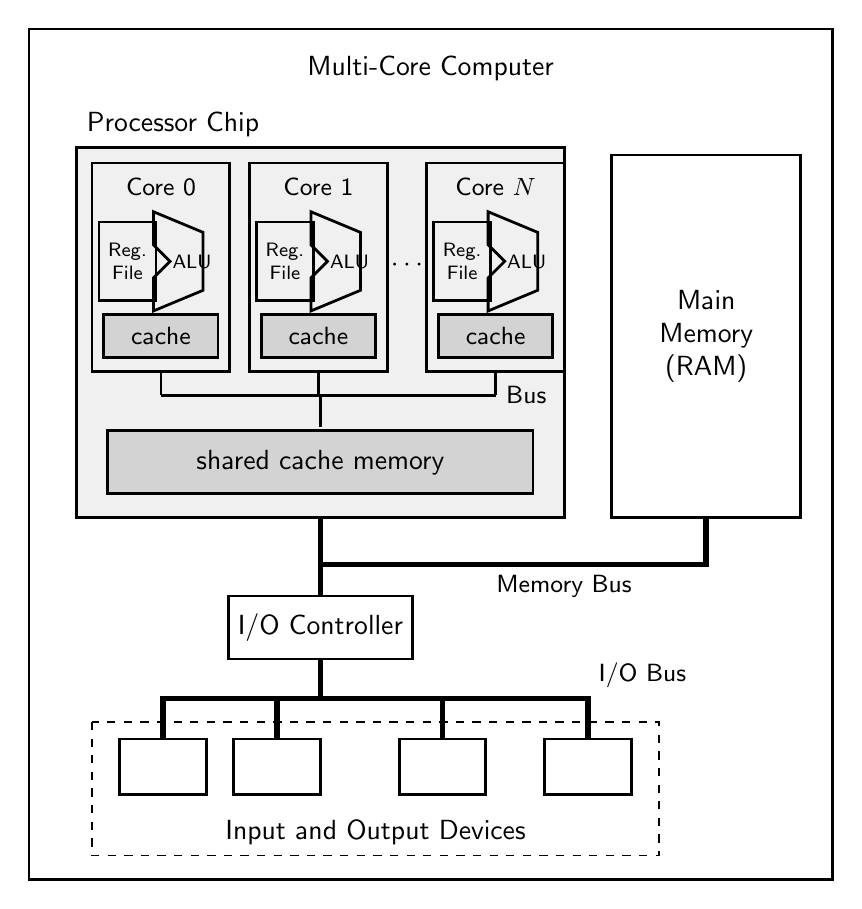
\begin{tikzpicture}[box/.style={draw, minimum height=0.8cm}]
  \newcommand{\alu}[1]{\draw[shift={(#1)}, scale=1.05] (0, 0) ++(-0.4, 0.6) -- ++(0.6, -0.25) -- ++(0, -0.7) -- ++(-0.6, -0.25) -- ++(0, 0.4) -- ++(0.2, 0.2) -- ++(-0.2, 0.2) -- cycle;}
  \node at (4.9, -0.3) {Multi-Core Computer};
  \draw[fill=black, fill opacity=0.06] (0.4, -1.3) rectangle (6.6, -6) node[pos=0, above right, opacity=1] {Processor Chip};
  % Each core has its own registers, ALU, and private cache; the cores share a cache over a bus.
  \foreach \x/\name in {0.6/Core 0, 2.6/Core 1, 4.85/Core $N$} {
    \draw (\x, -1.5) rectangle ++(1.75, -2.65);
    \node[font=\small] at (\x + 0.875, -1.8) {\name};
    \node[box, align=center, font=\scriptsize, minimum width=0.65cm, minimum height=1cm] at (\x + 0.45, -2.75) {Reg. \\ File};
    \alu{\x + 1.2, -2.75}
    \node[font=\scriptsize] at (\x + 1.27, -2.75) {ALU};
    \node[box, hl, font=\small, minimum width=1.45cm, minimum height=0.55cm] at (\x + 0.875, -3.7) {cache};
    \draw (\x + 0.875, -4.15) -- (\x + 0.875, -4.45);
  }
  \node at (4.6, -2.8) {$\cdots$};
  \draw (1.475, -4.45) -- (5.725, -4.45);
  \draw (3.5, -4.45) -- (3.5, -4.85);
  \node[right, font=\small] at (5.725, -4.45) {Bus};
  \node[box, hl, minimum width=5.4cm] at (3.5, -5.3) {shared cache memory};

  % Buses: the chip and main memory share the memory bus; devices hang off the I/O bus.
  \node[box, minimum width=2.4cm, minimum height=4.6cm, align=center] (ram) at (8.4, -3.7) {Main \\ Memory \\ (RAM)};
  \draw[line width=2pt] (3.5, -6) -- (3.5, -6.6) -| (ram.south);
  \node[below right, font=\small] at (5.6, -6.6) {Memory Bus};
  \node[box] (io) at (3.5, -7.4) {I/O Controller};
  \draw[line width=2pt] (3.5, -6.6) -- (io.north);
  \draw[line width=2pt] (io.south) -- (3.5, -8.3);
  \draw[line width=2pt] (1.5, -8.8) |- (6.9, -8.3) -- (6.9, -8.8);
  \foreach \x in {2.95, 5.05} \draw[line width=2pt] (\x, -8.3) -- (\x, -8.8);
  \node[above right, font=\small] at (6.9, -8.3) {I/O Bus};
  \foreach \x in {1.5, 2.95, 5.05, 6.9} \node[box, minimum width=1.1cm, minimum height=0.7cm, anchor=north] at (\x, -8.8) {};
  \draw[thin, dashed] (0.6, -8.6) rectangle (7.8, -10.3);
  \node at (4.2, -10) {Input and Output Devices};
  \draw (-0.2, 0.2) rectangle (10, -10.6);
\end{tikzpicture}
\end{document}
